% 색상 정의
\definecolor{coverblue}{RGB}{0, 74, 173}

\begin{tikzpicture}[remember picture, overlay]
    % 상단 파란색 박스
    \fill[coverblue] (current page.north west) rectangle ([yshift=-4cm]current page.north east);
    % 중앙 흰색 박스 (테두리 있음)
    \draw[line width=1pt, rounded corners=10pt, fill=white] 
        ([shift={(2cm,-6cm)}]current page.north west) 
        rectangle 
        ([shift={(-2cm,6cm)}]current page.south east);
\end{tikzpicture}

\begin{center}
    \thispagestyle{empty}
    {\fontsize{28}{34}\selectfont\textbf{\textcolor{white}{ABSTRACT(임시)}}}
    \vspace*{4.5cm}

    \begin{minipage}{0.85\textwidth}
        \begin{quote}
            \setlength{\parskip}{0.5em}
            본 연구는 군집 분석을 통해 학생들의 특징을 분석하고, 이를 바탕으로 학생들이 행복하게 느끼는 요소를 도출하는 것을 목표로 한다. 데이터 전처리 과정에서 결측치 처리 및 이상치 제거를 수행하였으며, KMeans 알고리즘을 사용하여 군집화를 진행하였다. 군집화 결과를 시각화하여 각 군집의 특징을 분석하고, 이를 통해 학생들이 행복하게 느끼는 요소를 도출하였다.
        \end{quote}
    \end{minipage}

    \vspace{0.5cm}

    \begin{minipage}{0.85\textwidth}
        \begin{quote}
            \setlength{\parskip}{0.5em}
            \textbf{keywords:} 보고서, 완성되면, ai 돌려서, 완성할 페이지
        \end{quote}
    \end{minipage}

    \vspace{0.5cm}

    \begin{figure}[h]
        \centering
        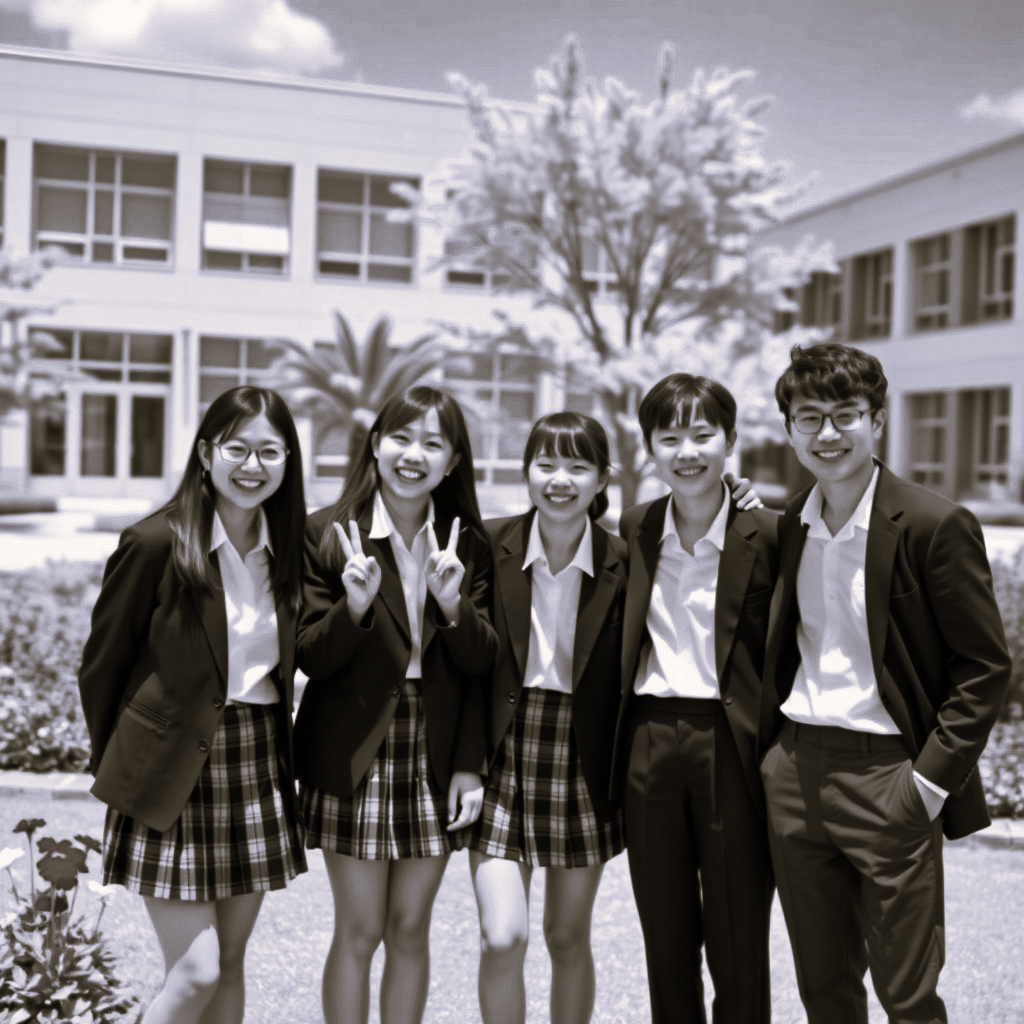
\includegraphics[width=0.7\textwidth]{img/2025-05-10-13-58-38.png}
        \caption*{\small 일단 임시로 넣어둔 이미지}
    \end{figure}
\end{center}
